\section{Mechanizm budowania (Bogna Lew)}

Opracowany mechanizm umożliwia graczowi na przełączenie się w tryb budowania poprzez naciśnięcie klawisza "B", który od razu
wyświetli podgląd bazowego obiektu. Widok budynku przemieszcza się przed postacią oraz odpowiednio obraca się razem z
nią. Efekt poruszania się podglądu został uzyskany za pomocą poniższych wzorów:
\begin{equation*}
\begin{cases}
x = r \times sin(\alpha) \\
y = 0 \\
z = r \times cos(\alpha)
\end{cases}
\end{equation*}

gdzie $r$ to odległość środka obiektu od postaci gracza, natomiast $\alpha$ to kąt o jaki jest on obrócony względem osi y.

Podgląd budynku będzie widoczny do czasu, aż gracz go umieści naciskając prawy przycisk myszy bądź wychodząc z trybu
edycji naciskając klawisz Escape. Jeżeli widok budowli znajduje się w poprawnym do umieszczenia miejscu to jest on
podświetlany na zielono, w przeciwnym razie - na czerwono. Wybudowanie powoduje przywrócenie bazowych kolorów obiektu
oraz włącza wykrywanie kolizji z nim, dzięki czemu budynek poprawnie oddziałuje z otaczającym go środowiskiem.

\begin{figure}[h!]
    \centering
    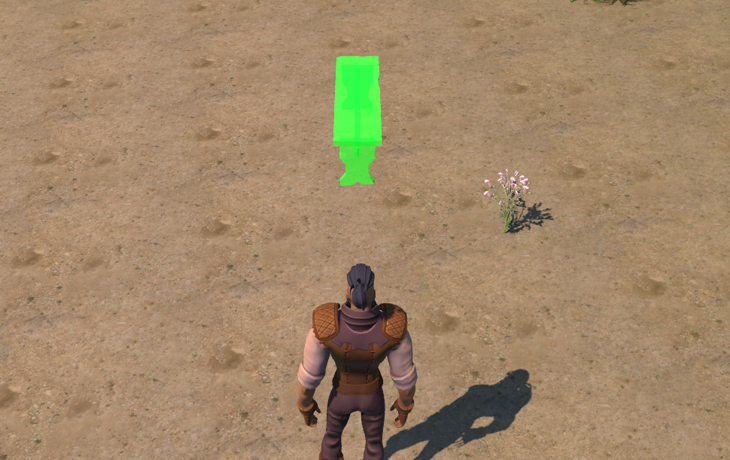
\includegraphics[width=0.9\textwidth]{images/implementacja/mechanizm_budowania/poprawne.png}
    \caption{Przykład podglądu w poprawnym umiejscowieniu.}
\end{figure}

Do weryfikacji poprawności umiejscowienia budynku wykorzystano mechanizmy wyzwalacza (ang. \textit{trigger}) oraz rzucania
promienia (ang. \textit{raycasting}). Pierwszy z nich polega na wykrywaniu czy obiekt znalazł się w obszarze kolizji bez
brutalnego zatrzymywania go. Oznacza to, że może on przeniknąć przez inny element bez widocznych konsekwencji, jedynie
wysyłając sygnał, że dana sytuacja nastąpiła. Druga metoda natomiast polega na wypuszczeniu promienia o pewnej długości
w zadanym kierunku i sprawdzeniu, czy z czymś się zderzył.

Wyzwalacz został zastosowany do wykrywania kolizji z innymi obiektami na mapie takimi jak postacie, czy elementy
scenerii niebędące terenem. W tym celu wykorzystano metody \textit{OnTriggerEnter()} i \textit{OnTriggerExit()}, które są wywoływane
odpowiednio gdy, dany obiekt znalazł się w obszarze kolizji innego elementu, bądź go opuścił. Każda z nich odpowiednio
zmienia poprzez inkrementację bądź dekrementację licznika kolizji obiektu. Jeżeli jego wartość jest różna od zera, tzn.
obiekt z czymś koliduje, to umiejscowienie jest uznawane za niepoprawne.

Drugi z mechanizmów został wykorzystany do sprawdzenia nachylenia podłoża. Efekt został osiągnięty poprzez rzucenie
promienia o niewielkiej długości z każdego z dolnych narożników obiektu i zliczeniu ile z nich wykryło kolizję z ziemią.
Brak wykrycia kolizji można zinterpretować jako zapadanie się bądź zbyt mocne lewitowanie danego narożnika nad
powierzchnią ziemi. Z tego powodu przyjęto, że jeśli co najmniej trzy z nich zderzyły się z podłożem, to umiejscowienie
jest poprawne.

\begin{figure}[h!]
    \centering
    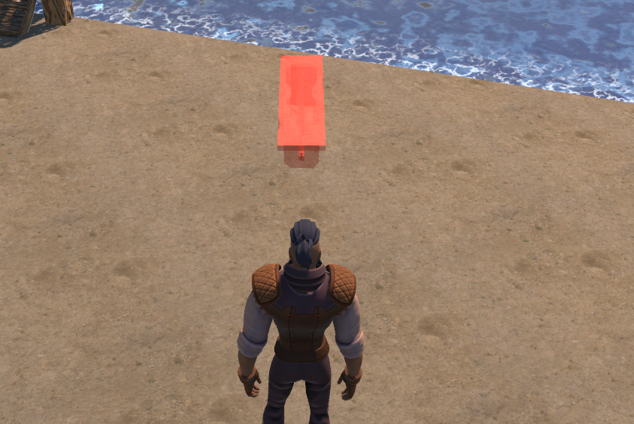
\includegraphics[width=0.9\textwidth]{images/implementacja/mechanizm_budowania/niepoprawne.png}
    \caption{Przykład podglądu w niepoprawnym umiejscowieniu.}
\end{figure}

Dodatkowo metodę rzucania promienia wykorzystano do wykrycia kolizji z drzewami. Obiekty te są traktowane przez silnik
jako część terenu, przez co metoda wykorzystująca wyzwalacz pomija je. Dlatego w celu wykrywania kolizji z nimi
zdecydowano się na rzucenie dwóch grup promieni biegnących w głąb obiektu z naprzeciwległych krawędzi prostopadłych do
osi y. Każdy z promieni biegnie w połowie wysokości obiektu i sięga przeciwnej ściany. Tak skomplikowany układ ma na
celu zapewnienie poprawności wykrywania kolizji w przypadku, gdy początki promieni znajdują się wewnątrz kolidującego
obiektu. Jeśli którykolwiek z nich zderzy się z drzewem, to wybrane miejsce jest uznawane za niepoprawne.

\begin{figure}[h!]
   \centering
   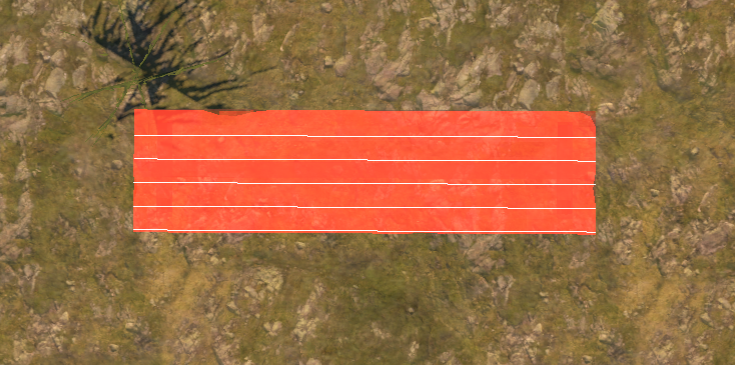
\includegraphics[width=.8\textwidth]{images/implementacja/mechanizm_budowania/gizmos_drzewo_2.png}
   \caption{Widok z góry na siatkę promieni służących do wykrywania kolizji z drzewami.}
\end{figure}
\begin{figure}[h!]
   \centering
   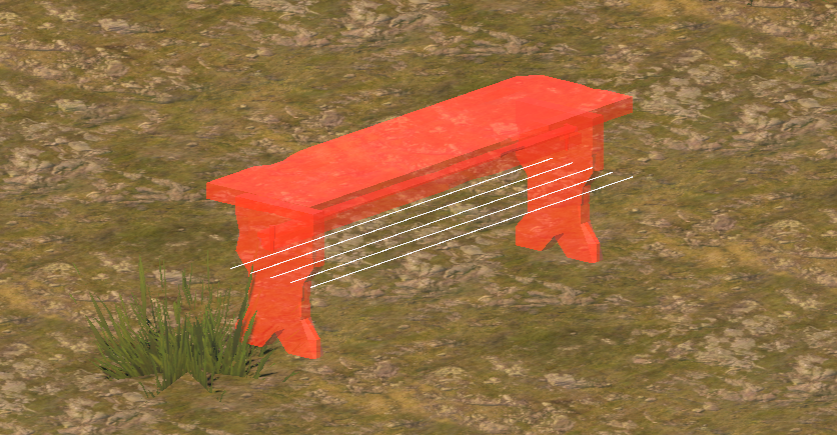
\includegraphics[width=.8\textwidth]{images/implementacja/mechanizm_budowania/gizmos_drzewo_1.png}
   \caption{Widok z boku na siatkę promieni służących do wykrywania kolizji z drzewami.}
\end{figure}
\FloatBarrier
